\documentclass[11pt]{beamer}
\usetheme{Warsaw}
\usepackage[utf8]{inputenc}
\usepackage{amsmath}
\usepackage{amsfonts}
\usepackage{amssymb}
\usepackage{tikz}
\usetikzlibrary{arrows,automata}
%\usepackage[latin1]{inputenc}

\author{Team Expeditus}
\title{UAV Autonomous Landing}
%\setbeamercovered{transparent} 
%\setbeamertemplate{navigation symbols}{} 
%\logo{} 
\institute{Dept. of Computer Science, SDSMT} 
%\date{} 
%\subject{} 
\begin{document}

\begin{frame}
\titlepage
\end{frame}

%\begin{frame}
%\tableofcontents
%\end{frame}

\begin{frame}{Team}
\textbf{Team Expeditus}\\
Jonathan Dixon, Dylan Geyer, Christopher Smith, Steven Huerta\\ 
\vspace{6mm}
\textbf{Sponsor}\\
Dr. Larry Pyeatt\\
\vspace{6mm}
\textbf{Goal}\\
Software to autonomously take-off, navigate to set waypoints, return to launch pad, and land
\end{frame}

\begin{frame}{Phase Objectives}
\textbf{Phase I}
\begin{itemize}
\item Build UAV 
\item Flight Controller Operating Correctly
\item Simulation Environment Available
\end{itemize}
\vspace{5mm}
\textbf{Phase II}
\begin{itemize}
\item Autonomous landing ready for simulation
\item Autonomous landing ready for UAV
\end{itemize}
\end{frame}

\begin{frame}{Testing}
\textbf{Phase I}
\begin{itemize}
\item Manual Flight of UAV
\item Autonomous Flight of UAV 
\end{itemize}
\vspace{5mm}
\textbf{Phase II}
\begin{itemize}
\item Autonomous Landing in Simulation
\item Autonomous Landing of UAV
\item Autonomous Take-off, Navigation, and Landing of UAV
\end{itemize}
\end{frame}

\begin{frame}{Approach - UAV}

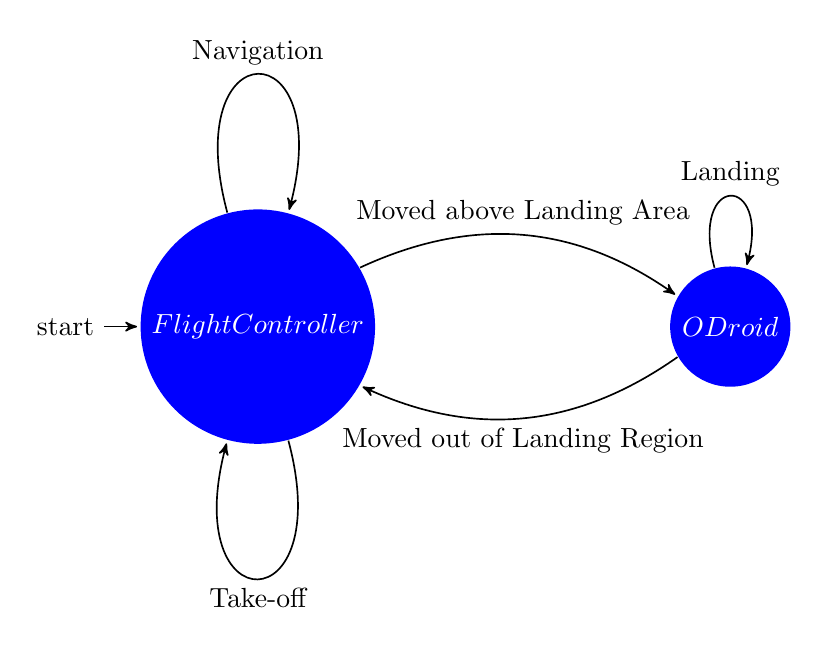
\begin{tikzpicture}[->,>=stealth',shorten >=1pt,auto,node distance=6cm,
                    semithick]
  \tikzstyle{every state}=[fill=blue,draw=none,text=white]

  \node[initial,state] (A)              {$Flight Controller$};
  \node[state]         (B) [right of=A] {$ODroid$};

  \path (A) edge [loop below] node {Take-off} (A)
            edge [loop above]  node {Navigation} (A)
            edge [anchor=center,bend left,above] node {Moved above Landing Area} (B)
        (B) edge [loop above] node {Landing} (B)
            edge [anchor=center,bend left,left,below]  node {Moved out of Landing Region} (A);
\end{tikzpicture}
\end{frame}

\begin{frame}{Approach - Software}
\begin{figure}
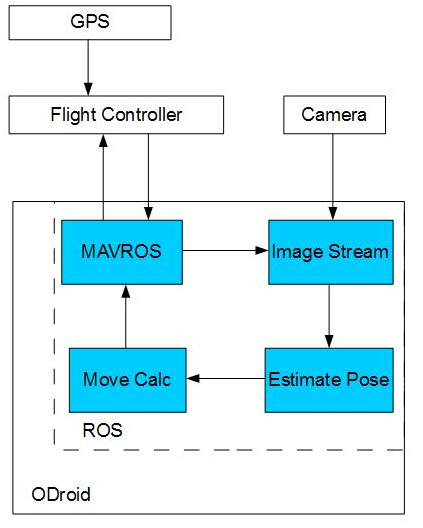
\includegraphics[width=.5\textwidth]{broad_approach1}
\end{figure}
\end{frame}

\begin{frame}{Approach - Landing Vision}
Put some stuff here about the landing vision approach, maybe a picture or two
\end{frame}

\begin{frame}{Approach - Landing AI}
\textbf{Artificial Neural Network (ANN) Approach}:
\begin{itemize}
\item Use Flight Controller to reach landing pad waypoint
\item Switch to landing mode using ANN
\item Land on landing pad or get within some distance to switch to vision
\end{itemize}
\end{frame}


\begin{frame}{Development - Software}
\textbf{Development OS}: Ubuntu 14.04\\
\textbf{Language}: C++\\
\vspace{5mm}
\textbf{Software Tools}
\begin{itemize}
\item Robot Operating System(ROS)
\item Gazebo
\item APM Planner
\end{itemize}
\end{frame}


\begin{frame}{Development - Software Contd.}
\textbf{Simulation \& Testing}: 
\begin{itemize}
\item Rotors Sim package - Provides Models for Gazebo
\end{itemize}
\centerline{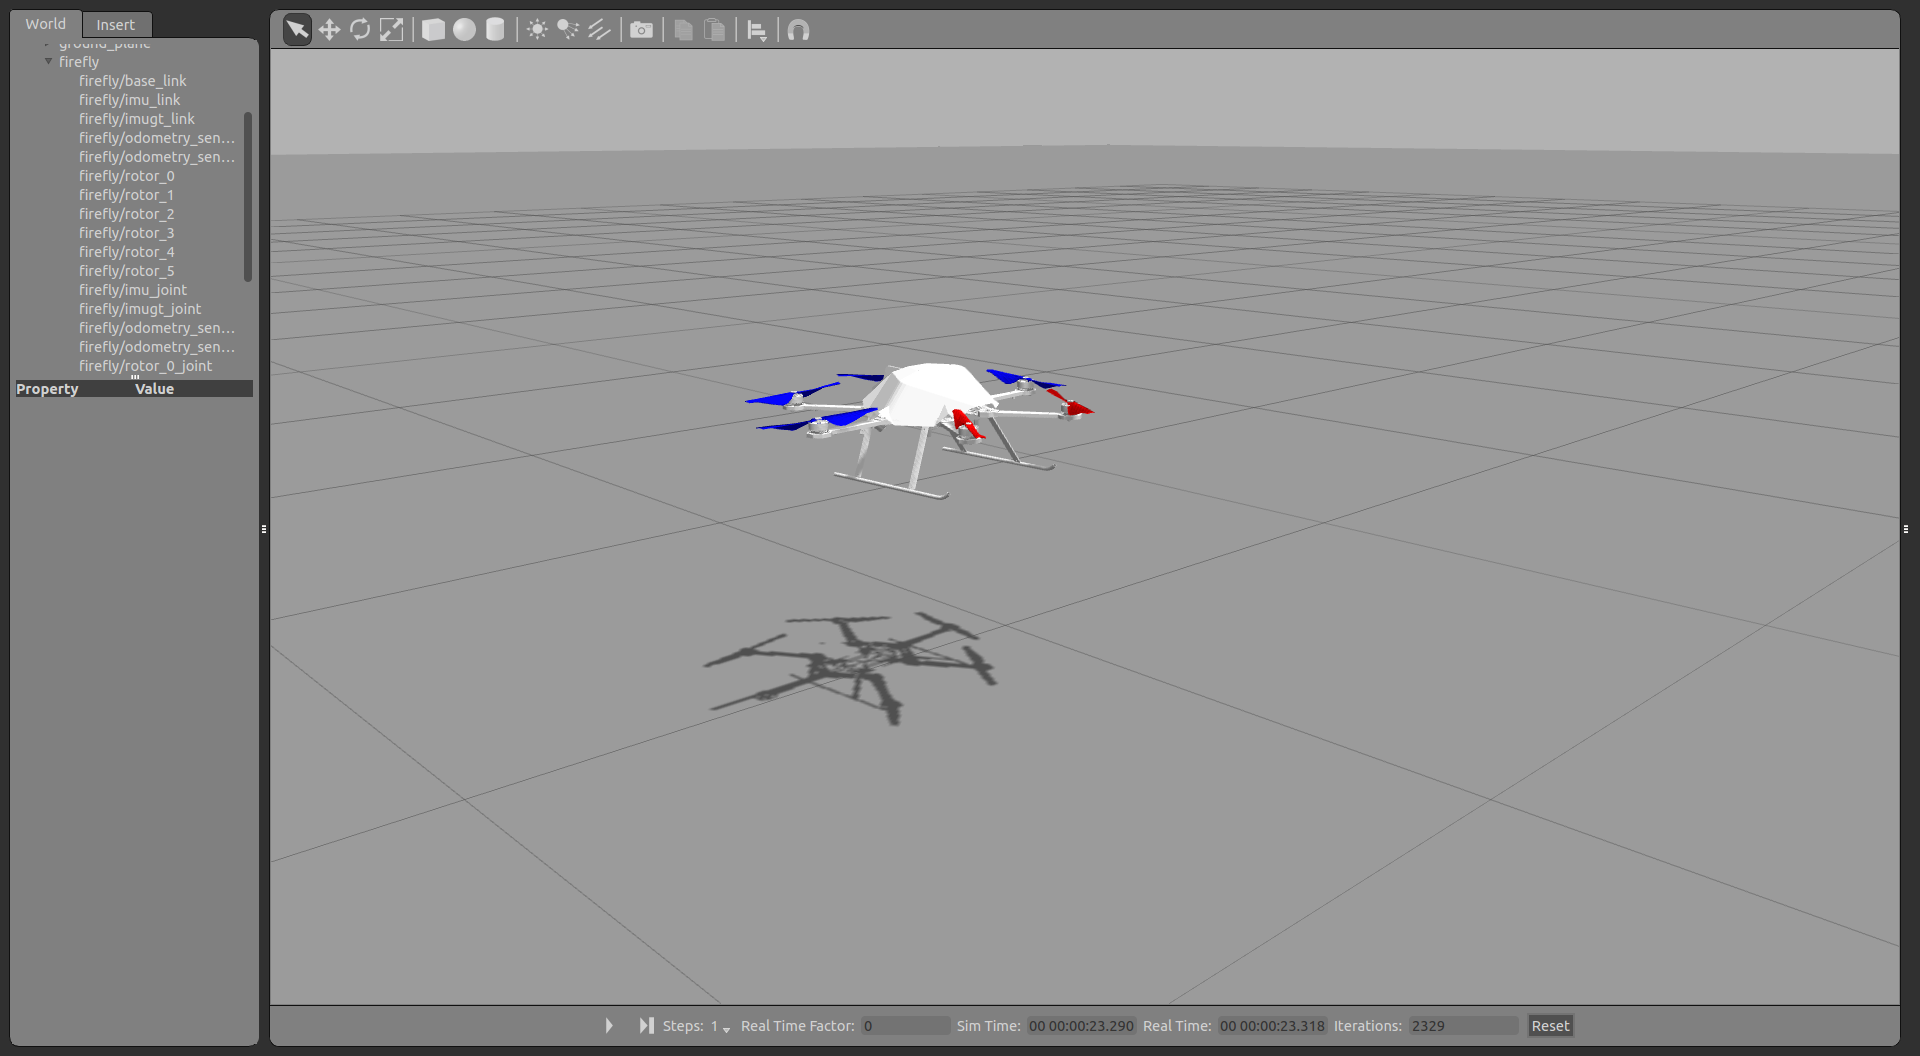
\includegraphics[scale=0.15]{images/Gazebo_Joy.png}}
\end{frame}

\begin{frame}{Development - Software Contd.}
\begin{itemize} 
\item MavRos - Communication with Pixhawk through ROS
\item Testing - All components will be tested in simulation before being deployed on UAV
\end{itemize}
\centerline{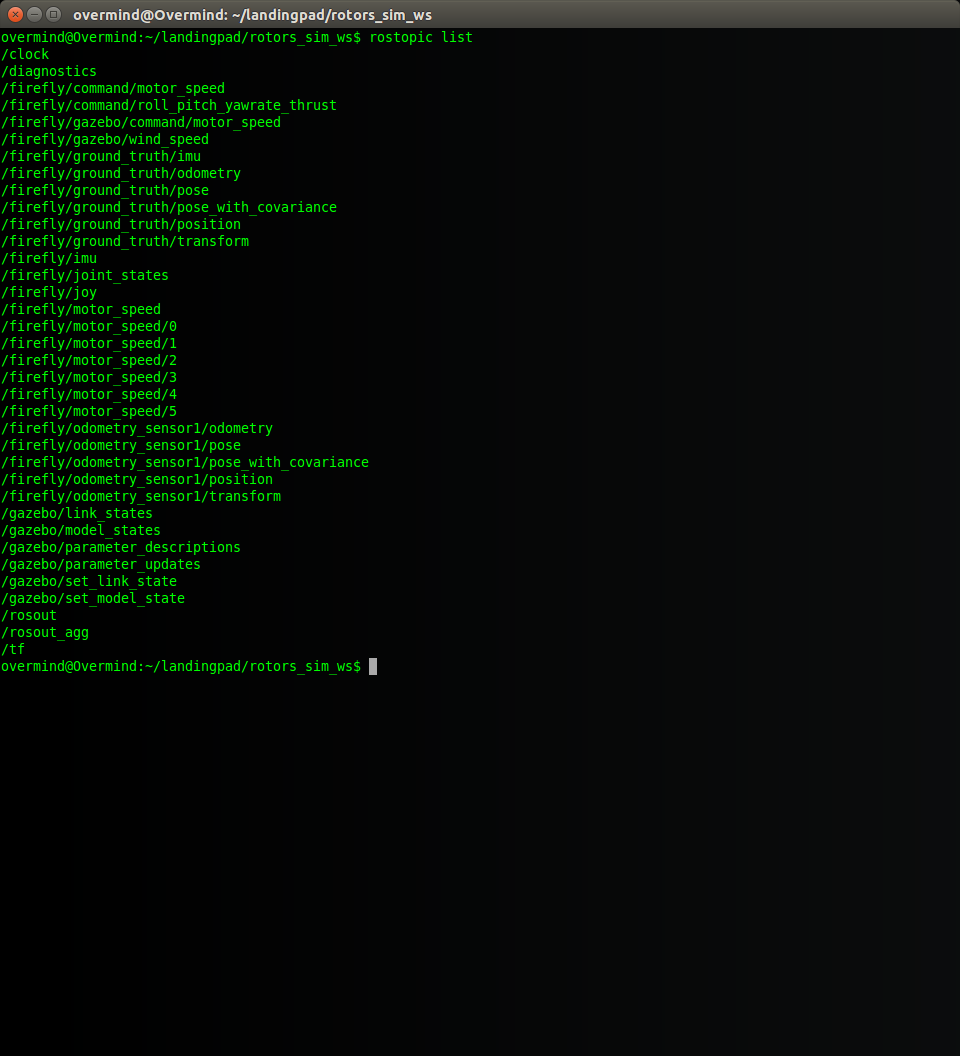
\includegraphics[scale=0.15]{images/Ros_Topics.png}}
\end{frame}

\begin{frame}{Development - Hardware}
\textbf{Hardware Constraints}
\begin{itemize}
	\item 6000mAh Battery
	\item Power ODroid + Peripherals
	\item Power 6x DC Motors
\end{itemize}

\centerline{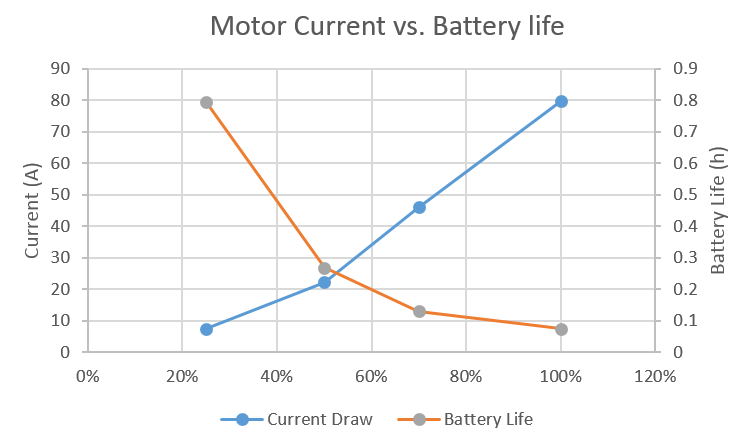
\includegraphics[width=0.75\textwidth]{Power_BatteryLife}}

\end{frame}

\begin{frame}{Development - Hardware Continued...}

	\begin{tabular}[c]{| c | c | c |}
		\hline
		Item & Quantity & Total Weight\\
		\hline
		DC Motor & 6 & 372g\\
		\hline
		Frame & 1 & 1300g\\
		\hline
		Battery & 1 & 680g\\
		\hline
		Camera & 2 & 140g\\
		\hline
		ODroid & 1 & 48g\\
		\hline
		GPS Module & 1 & 17g\\
		\hline
		\multicolumn{2}{| r |}{\textbf{Total}} & 2557g\\
		\hline
	\end{tabular}
	\hfill \break \\
	1 Motor at 100\% produces 970g of lift\\
	Maximum Lift = 5820g\\
	Motors must run at 2557g / 5820g = 44\%
\end{frame}

\begin{frame}{Development - Hardware Continued...}
	\textbf{Computational Constraints}
	\begin{itemize}
		\item Images: 976 x 582 pixels at $\ge$ 5 images/sec
		\item Processing 1 image thus requires $\sim$570,000 operations
		\item ODroid has 8 cores at 1.4 GHz
		\begin{itemize}
			\item Ideal throughput $\sim$10 Billion operations/sec
		\end{itemize}
	\end{itemize}
\end{frame}

\begin{frame}{Cost}
\centering{
\begin{tabular}[c]{| l | r | l | r |}
\hline
\multicolumn{2}{| c |}{\textbf{Build 1}} & \multicolumn{2}{| c |}{\textbf{Build 2}} \\
\hline
Item & Cost & Item & Cost \\
\hline
Controller & \$199.99 & Controller & \$199.99\\
\hline
ODroid 	   & \$75.95  & ODroid 	   & \$75.95 \\
\hline
Sensors    & \$167.23 & Sensors    & \$167.23 \\
\hline
Frame Kit  & \$242.48 &  &\\
\hline
Power Kit  & \$119.98 &  &\\
\hline
Radio Set  & \$100.00 &  &\\
\hline
Extra Parts & \$95.15 &  &\\
\hline
\textbf{TOTAL} & \$1000.78 & \textbf{TOTAL} & \$443.17\\
\hline
\end{tabular}
}
\end{frame}

\begin{frame}{Work Accomplished}
\textbf{General}
\begin{itemize}
\item Review previous iteration documentation \& code
\item Begin pilot training for manual control
\item Review Landing Pad model with Landing Pad teams
\end{itemize}
\vspace{4mm}
\textbf{Setup Development Environment}
\begin{itemize}
\item Ubuntu 14.04
\item Gazebo/Rviz
\item ROS - Jade Distro
\end{itemize}
\vspace{4mm}
\textbf{Inspect Current Quadrotor}
\begin{itemize}
\item Identify missing or non-functioning components 
\item Generate order list
\end{itemize}
\end{frame}

\begin{frame}{Setbacks/Risk}
\textbf{Risk}
\begin{itemize}
\item Reliance on Flight Controller
\item Dependency on external team for Landing Pad
\item No UAV Backup
\end{itemize}
\vspace{6mm}
\textbf{Setbacks}
\begin{itemize}
\item Non-functional components
\item Little carry-over from previous year
\end{itemize}
\end{frame}

\begin{frame}{Conclusion}
Conclusion-y stuff here
\end{frame}

\begin{frame}
\center \Large{{\textbf{Questions?}}}
\end{frame}

\end{document}
